\documentclass[a4paper,11pt]{article}

\usepackage[utf8]{inputenc}	
\usepackage[T1]{fontenc}
\usepackage{lmodern}
\usepackage{times}
\usepackage[margin=2cm]{geometry}
\usepackage{amsmath}
\usepackage{mathtools}
\usepackage{graphicx}
\usepackage{multirow}
\usepackage{blindtext}
\usepackage{hyperref}

\usepackage{pgfplotstable} 
\usepackage{booktabs}

\graphicspath{ {./images/} }

\usepackage[czech]{babel}
\usepackage{graphicx}
\usepackage{amsmath}
\usepackage{xspace}
\usepackage{url}
\usepackage{indentfirst}
\usepackage{listings}
\usepackage{subcaption}
\usepackage{caption}
\usepackage{tabularx}
\usepackage[labelformat=parens,labelsep=quad,skip=3pt]{caption}

\widowpenalty 10000 \clubpenalty 10000 \displaywidowpenalty 10000
\setcounter{topnumber}{3}	  
\setcounter{bottomnumber}{3}	 
\setcounter{totalnumber}{6}	  
\renewcommand\topfraction{0.9}	 
\renewcommand\bottomfraction{0.9} 
\renewcommand\textfraction{0.1}	  
\intextsep=8mm \textfloatsep=8mm 

\renewcommand{\thesection}{\arabic{section}.}
\renewcommand{\thesubsection}{\thesection\arabic{subsection}.}
\makeatletter \def\@seccntformat#1{\csname the#1\endcsname\hspace{1ex}} \makeatother

\begin{document}

\hline
\begin{center}
\bigskip
\huge Světelná křivka proměnné hvězdy
\vspace{0.5cm}
\par \large F3190: Praktikum z astronomie 1
\par \large Artem Gorodilov
\vspace{0.5cm}
\par \large 12. ~března 2024
\bigskip
\end{center}
\hline
\bigskip


\vskip10pt
    \begin{minipage}[t]{0.5\textwidth} 
        \section{Abstrakt}    
            V této práci jsme zkoumali fotometrická data proměnné hvězdy. Ze série 22 snímků pořízených po dobu 3,5 hodiny každých 10 minut jsme pomocí Pogsonova zákona získali světelnou křivku proměnné hvězdy. Ze snímků jsme vybrali hvězdy A,B a C (viz níže), pro které jsme provedli výpočty jasnosti, které byly následně použity k výpočtu zdánlivé hvězdné velikosti proměnné hvězdy. 
            \par Výpočty jsme se snažili provádět automatizovanou metodou pomocí pythonové pipeline napsané speciálně pro tento problém. Porovnali jsme ji také s klasickou metodou určování hvězdné velikosti Luboš Brát, 1998\cite{brat1998}
        \section{Teorie}
            \subsection{Pogsonův zákon}
                \par Pogsonův zákon je metoda používaná pro kalibraci magnitudy proměnné hvězdy na základě každé srovnávací hvězdy je základní formou diferenciální fotometrie. Při diferenciální fotometrii se magnituda cílového objektu (v tomto případě proměnné hvězdy) určuje vzhledem k jedné nebo více srovnávacím hvězdám se známou magnitudou. Tento přístup pomáhá zmírnit vliv atmosférických změn, změn citlivosti přístrojů a dalších faktorů, které mohou ovlivnit pozorovanou jasnost nebeských objektů.
                \par Vztah mezi jasností a hvězdnou velikostí je dán Pogsonovým zákonem:
                \begin{equation}
                    m_1 - m_2 = -2.5 \log \left( \frac{I_1}{I_2} \right)
                \end{equation}
                kde $m_1$ a $m_2$ jsou hvězdné velikosti dvou hvězd a $I_1$ a $I_2$ jsou jejich jasnosti.
    \end{minipage}
    \hspace{10pt}
    \begin{minipage}[t]{0.5\textwidth} 
        \section{Zpracování dat}в
            \subsection{Popis paipelinu}
                Jako vstupní data jsme dostali 22 snímků noční oblohy modelovaných pomocí softwaru TRENAŽÉR pro datum 27.2.2024 mezi 18:30 (UT) a 22:00 (UT). 
                \par K dispozici máme hvězdné velikosti tří hvězd (A, B a C), se kterými budeme porovnávat změnu jasnosti proměnné hvězdy (obr. 1).
                
                \vspace{10pt}   
                \par \centering
                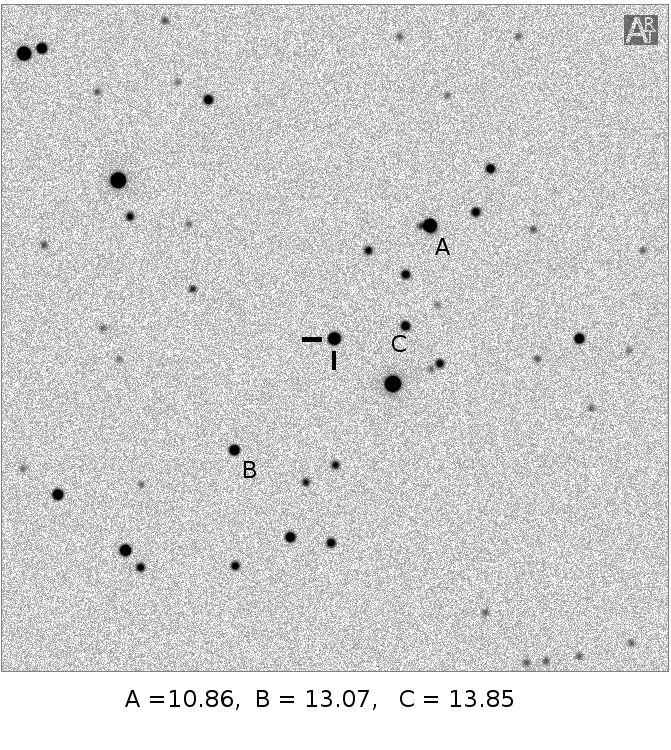
\includegraphics[scale=0.3]{art_note}
                \captionsetup{justification=centering, font=footnotesize}
                \captionof{figure}{Snímek noční oblohy s označenými hvězdami A, B a C. Proměnná hvězda je označena křížkem.}
                \label{fig:art_note}
                \vspace{10pt}
                \raggedright  
                
                \par Pro automatizaci analýzy a získání světelných křivek z 22 snímků, které nám byly poskytnuty, jsme použili pipeline, která zpracovává data pomocí knihoven: \texttt{cv2}, \texttt{photutils} a \texttt{astropy}. 
                \par Podstatou naší metody je určení jasnosti na základě analýzy obrázku .png, kde na vybrané oblasti obrázku bude zkonstruována apertura a prstenec o určitých poloměrech (obr. 2), 

    \end{minipage}

\newpage
    \begin{minipage}[t]{0.5\textwidth} 
                \vspace{10pt}   
                \par \centering
                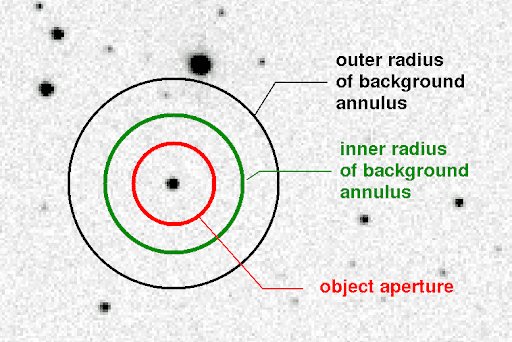
\includegraphics[scale=0.4]{apert}
                \captionsetup{justification=centering, font=footnotesize}
                \captionof{figure}{Vizualizace apertury a prstence pro výpočet jasnosti hvězdy.}
                \label{fig:apert}
                \vspace{10pt}
                \raggedright 
                
                \par poté pomocí funkce \texttt{measure\_brightness()} vypočítáme jasnost vybraných hvězd pro každý obrázek. Poté pomocí Pogsonova zákona vypočítáme hvězdnou velikost proměnné hvězdy a sestrojíme její světelnou křivku pro případy porovnání se třemi hvězdami zvlášť. 

            \subsection{Hlavní kroky paipelinu}
                \par Aby bylo možné spustit Pipeline, je třeba do ní načíst obrázky a vložit k nim cestu do proměnné \texttt{image\_paths}, poté obrázky převést na matici s intenzitou pixelů jako prvky pomocí \texttt{cv2}. 
                \par Určete polohy [x,y] v px pro tři hvězdy se známou hvězdnou velikostí (A, B, C) a polohu proměnné hvězdy a poté tyto hodnoty vložte do proměnné \texttt{position}.
                \par Nastavte poloměr apertury, vnitřní poloměr prstence a vnější poloměr prstence tak, že je vložíte do proměnných, \texttt{aperture\_radius}, \texttt{annulus\_inner\_radius} a \texttt{annulus\_outer\_radius}. 
                \par Do proměnné \texttt{mag\_comparisons} zapíšeme magnitudy nám známých hvězd ve stejném pořadí jako v \texttt{position}. 
                \par Dále pro každý snímek určíme jasnost těchto hvězd pomocí funkce \texttt{measure\_brightness()}, která kolem vybraných hvězd sestaví apertury a anuly a pomocí fotometrických výpočtů vrátí jasnosti těchto hvězd (obr. 3). 
                \par Posledním krokem bude výpočet magnitudy proměnné hvězdy pomocí Pogsonova zákona podle vzorce (1), kde $m_1$ bude naše proměnná hvězda a $m_2$ hvězda se známou hvězdnou velikostí. 
        \section{Výsledky}
                Po použití piplanu jsme získali tři světelné křivky pro proměnnou hvězdu (modrou, žlutou a zelenou),
    \end{minipage}
    \hspace{10pt}
    \begin{minipage}[t]{0.5\textwidth}
                \vspace{10pt}   
                \par \centering
                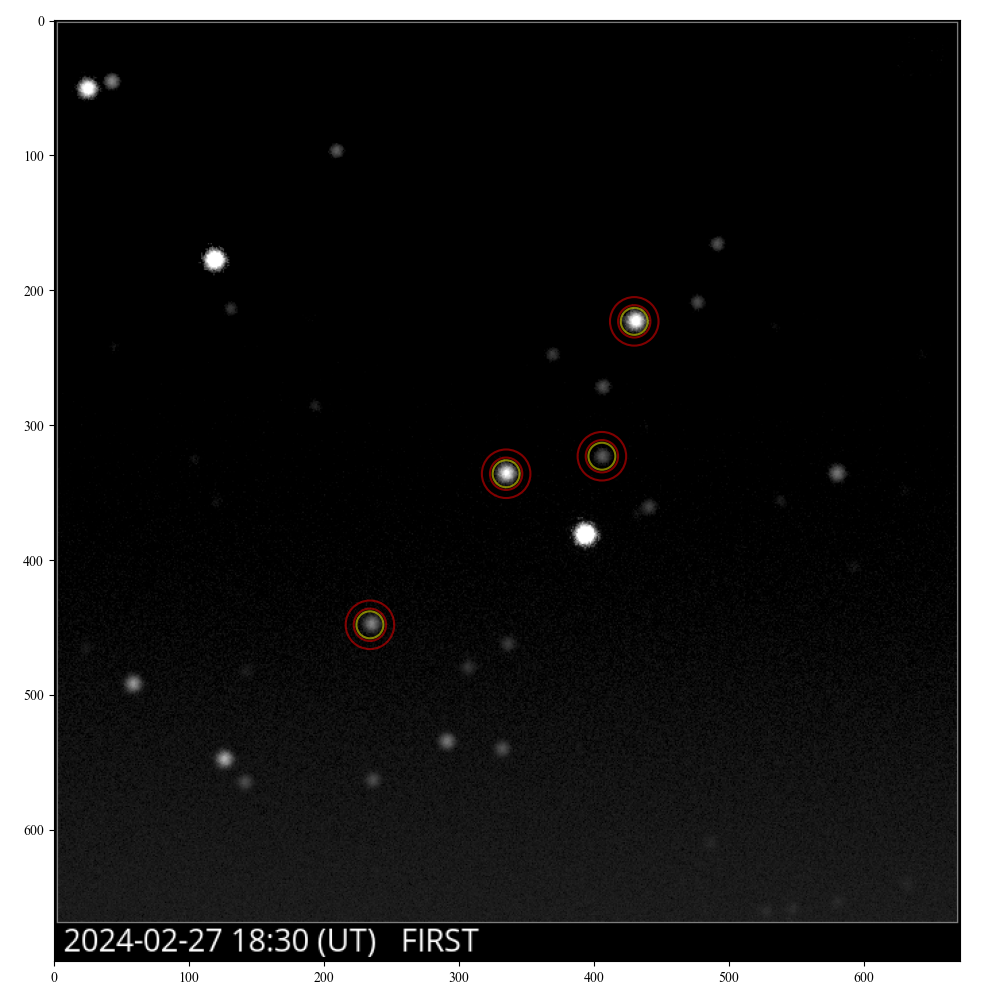
\includegraphics[scale=0.32]{apertures}
                \captionsetup{justification=centering, font=footnotesize}
                \captionof{figure}{Apertura a prstenec pro výpočet jasnosti hvězdy.}
                \label{fig:apert}
                \vspace{10pt}
                \raggedright 

                přičemž pro srovnání jsme použili vždy jednu z hvězd a známou hvězdnou velikost (A, B a C). 
                \par Pro každý pozorovací bod jsme vypočítali střední hodnotu hvězdné velikosti, kterou budeme brát jako výslednou světelnou křivku (červená).
                \par Pro srovnání jsme také použili klasickou metodu určování hvězdné velikosti, kterou jsme porovnali s výsledky z pipeline (fialová).

                \vspace{10pt}   
                \par \centering
                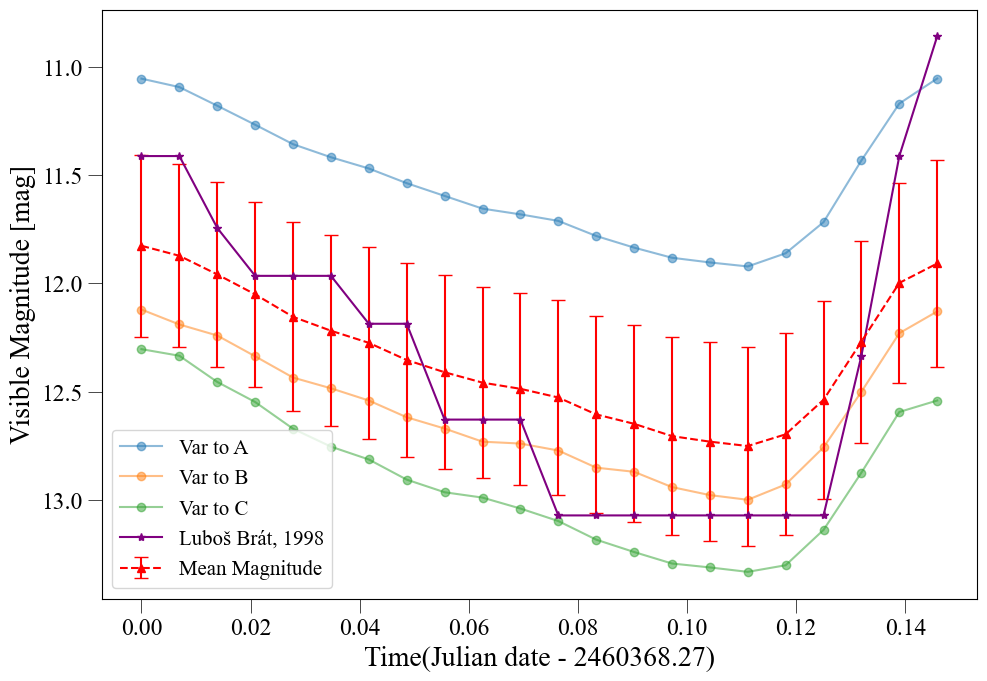
\includegraphics[scale=0.32]{lc}
                \captionsetup{justification=centering, font=footnotesize}
                \captionof{figure}{Světelné křivky pro proměnnou hvězdu.}
                \label{fig:apert}
                \vspace{10pt}
                \raggedright 
        \section{Závěr}
                Výsledky z pipeline se shodují s výsledky z klasické metody určování hvězdné velikosti. Pokud budeme uvažovat hlouběji, kromě velkých chyb, které lze vysvětlit kvalitou snímku, přesněji jeho formátem (.png místo .fits), je světelná křivka získaná pomocí Pipeline mnohem hladší a vhodnější pro další analýzu.  
                \par Výhodou pipeline je, že je možné ji použít pro velké množství dat a získat tak výsledky rychleji a s menší chybou. 
    \end{minipage}
\newpage    
            \begin{center}
                \subsection{Tabulka s vypočtenými magnitudami a koeficienty p a q}
                    \pgfplotstabletypeset[
                        col sep=comma, % Defines the separator, comma for CSV
                        string type, % Treats columns as strings (not math mode)
                        every head row/.style={before row=\toprule,after row=\midrule},
                        every last row/.style={after row=\bottomrule},
                    ]{output.csv} 
            \end{center}
\begin{thebibliography}{9}
    \bibitem{brat1998} 
        1. Luboš Brát, 1998. Available online: \url{http://var2.astro.cz/download/1311352160_trenazer_LVAur.pdf}
\end{thebibliography}
\end{document}